\section{Analysis Techniques}

\key{running time}{experimental analysis}{theoretical analysis}{primitive operations}{growth rate of running time}{Big-Oh}

		\defn{Data Structure}{is a systematic way of organising and accessing data}

		\defn{Algorithm}{is a step-by-step procedure for performing some task in a finite amount of data}

		\defn{Running Time}{is the amount of time it takes an algorithm to execute in full}

		\par{The main criteria used to compare different algorithms are running time and memory usage. In general the running time of an algorithm increases with the
		input size, and may vary depending on the hardware and software environments on which it is run. When comparing algorithms one aims to control those variables
		and express a relation between their run times and inputs via some function}

\subsection{Experimental Analysis vs Theoretical Analysis}

		\par{One way to study the efficiency of an algorithm is to run an empirical study. The dependent and independent variables are set, several trials are run a
		with appropriate inputs and then a statistical analysis is carried out on the output of the experiments.}

		%INSERT PLOT p.141

		%\caption{The plot above compares two algorithms for string concatenation in Java.}

		\par{\mymarginpar{Drawbacks}Though the experiment itself is relatively straightforward to run (once the algorithm is implemented), the analysis can be quite quite complicated to
		perform. Especially given that it can be hard to know which inputs are appropriate to use and , more importantly , given that fully implementing a complex algorithm is hard
		work and time-consuming. Hence, if possible a higher-level analysis is performed, if an algorithm can be deemed to be inferior by application of theoretical
		methods then no experimental analysis is required}


\par{So, when developing theoretical methods of analysis one's goal is to overcome the drawbacks mentioned above in order to achieve the following:}

\begin{enumerate}
	\item System Independence
	\item Input Coverage
	\item High-Level Description
\end{enumerate}


\defn{Primitive Operations}{are \ita{low-level} instructions with constant execution time (e.g. variable assignment, function call)}

\par{In order to express running time as a function of input size we use primitive operations, which are identifiable from abstract implementations (like
pseudocode) and taken to have a constant time of completion. In this way, one can compare the total number $t$ of ops for a given implementation, since by
assuming a constant time for all ops one can assume that the total running time will be \ita{proportional} to $t$}

\par{Ideally the average of all possible inputs would be used to characterize a given algorithm. However,finding the average often involves finding an
		appropriate distribution for the sample inputs. Hence, we characterize it instead in terms of its \ita{worst case} input which is far easier to
		identify. }
\rem{Another advantage is that minimising for the worst case by definition implies that we're optimising the running time for all other possible
inputs}

\subsection{Common Functions}

\par{This relation between input and running time is often expressed in terms of one of the following 7 functions}

\subsubsection{Constant}

	\par{The simplest function of them all is the constant function which simply
	assigns a given constant $c$ to any input $n$ . It is particularly useful,
	since it allows us to express the \ita{number of steps} needed to perform a basic
	operation}

	$$f(n) = c , \forall n \in \text{ input set }$$

	\rem{The essential constant functions if $g(n) = 1$ given that we can
	express any other constant function in the form $g(n)f(n)$}

\subsubsection{Logarithm}

	\par{The logarithmic function, in particular $\log_2$ , pops up all the
	time. A logarithmic runtime is characterized by larger differences in
	runtime for smaller inputs, with a significant decrease for larger inputs.}

	\defn{ceiling (of $x$)}{the smallest integer greater than x}

	\nota{$\lceil x \rceil$}

	\par{We can think of the ceiling function as an approximation of x. We can
			use it in a similar manner to approximate any given algorithm. By
			definition $\log_b(x)$ is just the power to which $b$ has to be
			raised to give $x$. Hence, we define $\lceil\log_b x\rceil$ as the
	smallest number for which $b$ has to be raised so that it includes $x$. So,
	we can divide repeatedly divide $x$ by $b$ until we get a number less or
	equal to 1}

	\ex{ $\lceil\log_{2}12\rceil = 4$ since $2^3 < 12 < 2^4$}

\subsubsection{Linear}

	\par{The linear function assigns the input to itself. It is useful to
	characterize single basic operations on $n$ elements}

	$$f(n) = n$$

\subsubsection{N-Log-N}

	\par{For any given input $n$ it assigns $n$ times $\log(n)$}

	$$f(n) = n\log(n)$$

\subsection{Quadratic}

	\par{The quadratic function appears primarily in algorithms with nested
			loops, since the inner loop performs an operation $n$ times and the
	outer loop will repeat each loop a \ita{linear} number of times}

	$$f(n) = n^2$$

\subsubsection{Polynomials}

\par{A more general class which subsumes the quadratic ($d=2$), linear ($d=1$)
		and constant ($d=0$) functions, where $d$ is the degree of the
		polynomial which corresponds to the largest exponent in the polynomial
		expression. In general, polynomials with lower degrees have better
running times}

$$f(n) = \sum_{i=0}^{d} a_{i}n^{i}$$

\subsubsection{Exponential}

	\par{Exponential time polynomials are generally the worst-case running time
			for an algorithm, since they grow very rapidly. As an example, take
			a loop which doubles the number of operations it performs with every
			iteration. Then, the total number of operations it performs will be
	$2^n$}


\subsection{Growth Rates}


	\par{If we take $f(n)$ to be the function which gives the total number of
			operations in the \ita{worst-case}, and $a\;z$ to be the time taken
			by the fastest and slowest primitive op , respectively. Then, the
			worst-case running time $T(n)$ for the algorithm is bounded by the two
	linear functions $af(n);zf(n)$ , i.e}

	$$af(n) \leq T(n) \leq bf(n)$$

	\par{Note that the growth rate of the worst-case running time is an
			intrinsic property of the algorithm which is not affected by by
	hardware or software environments. These factors affect $T(n)$ by a constant
	factor. Hence, when running an asymptotic analysis one can \textbf{disregard} constant
	and lower-degree terms}

	\rem{Ideally we want operations on data structures to run in times
			proportional to the constant or log functions, and algorithms to run
	in linear or n-log-n}

	\defn{Asymptotic Analysis}{analysing how the running time of an algorithm
			increases with the size of the input \ita{in the limit}, as the size
	of the input increases with the bound}

	\begin{figure}[H]
		\begin{center}
		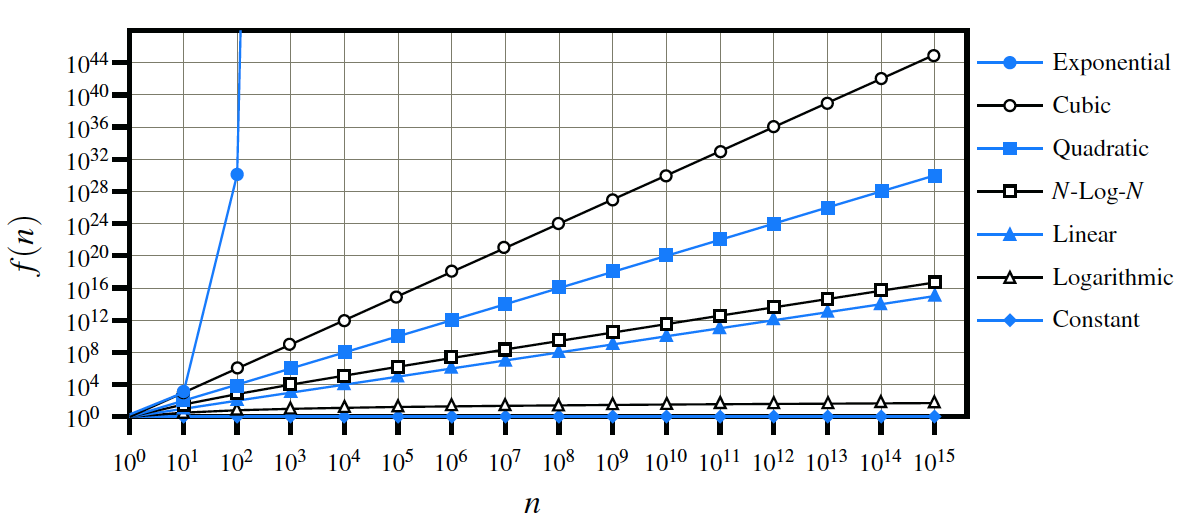
\includegraphics[width=\textwidth]{growth.png}
		\end{center}
	\end{figure}

\subsection{Big-Oh Notation}



		\defn{Big-Oh Notation}{we say that \ita{"$f(n)$ is big-Oh of $g(n)$"} if
		$\exists c \in \real s.t f(n) \leq cg(n)$ , for $n \geq n_0$}

		\notation{$f(n) is O\left(g(n)\right)$}
		\par{In essence we make use of the fact that growth run time is not affected by
				constant factors, and encode this into function notation. In effect
				bounding the function after a given input size $n_0$ by another
		function ; i.e $f(x)$ is strictly less than or equal to $g(x)$ up to to a
		constant factor and in the \ita{asymptotic sense}. Hence, we can use $g(x)$ to
		approximate/characterize $f(x)$}

		\par{We want this relation to be expressed in the simplest terms possible. Obviously it is easy to find such a function if one aims for the moon, i.e
				clearly $3n^2 + 2$ is $O(n^{10})$ this is however not very useful.
				Instead, simplifying the first expression by getting read of constant
				factors , we see that we can be sure that it is for sure $O(n^2) < O(n^{10})$,
		which is therefore a better approximation}

		\rem{We want the \ita{simplest} expression of the class of bounding functions
				($n^{2}$ Vs $4n^{2}$) and the \ita{smallest} possible class ($n^{2}$ Vs
		$n^{10}$)}

		\proposition{}{For any polynomial $p(n)$ of degree $d$ , $p(n) \in
		O\left(n^d\right)$}

		\proposition{}{$T_1(n) \in O(f(n)) , T_2(n) \in O(g(n)) \implies T_1(n)
		+ T_2(n) \in O(max(f(n),g(n)))$}

		\proposition{}{$T_{1}(n) \in O(f(n))$ and $T_{2}(n) \in O(g(n)) \implies
		T_{1}(n)T_{2}(n) = O(f(n)g(n))$}

		\proof{$T_{1}T_{2} = klf(n)g(n)$ , for constants $k,l$ . Hence, ignoring
		the constants we have the expected result}

		\prop{$T(n) = (\log n)^k \implies T(n) = O(n)$}

		\proof{$$T(n) \in O(f(n)) \iff \lim_{n\to\infty}(T(n) / f(n)) = 0)$$
		 \par{By \ita{L'Hopital's},  }$$lim_{n\to\infty}(f(n) / g(n)) =
				lim_{n\to\infty}(f\prime(n) / g\prime(n))$$

				\par{Take $f(n) = (\log n)^{k+1}$ and $g(n) = n$. Then, by
						induction on $k$ , $$(\log n)^1 = \log n \in O(n) \text{ and } (\log n)^k \in O(n)$$}

				\par{Hence, $$\lim_{n\to\infty}\left(\frac{(\log n)^{k+1}}{n}\right) = 0$$
						$$\lim_{n\to\infty}\left(\frac{(\log n)^{k+1}}{n}\right) =
				\lim_{n\to\infty}\left(\frac{(k+1)(\log n)^k}{n}\right) = 0$$}

				\par{Therefore, the result follows by induction}
		}
\subsection{Big-Omega \& Big-Theta}

		\defn{$\Omega\left(n\right)$}{$f(n) \geq cg(n)$}

		\defn{$\Theta\left(n\right)$}{$c\prime g(n) \leq f(n) \leq c\prime\prime g(n)$}

		\par{Similarly to $O\left(n\right)$ , these provide upper and upper+lower bounds
		respectively}


		\begin{figure}[H]
		\begin{center}
				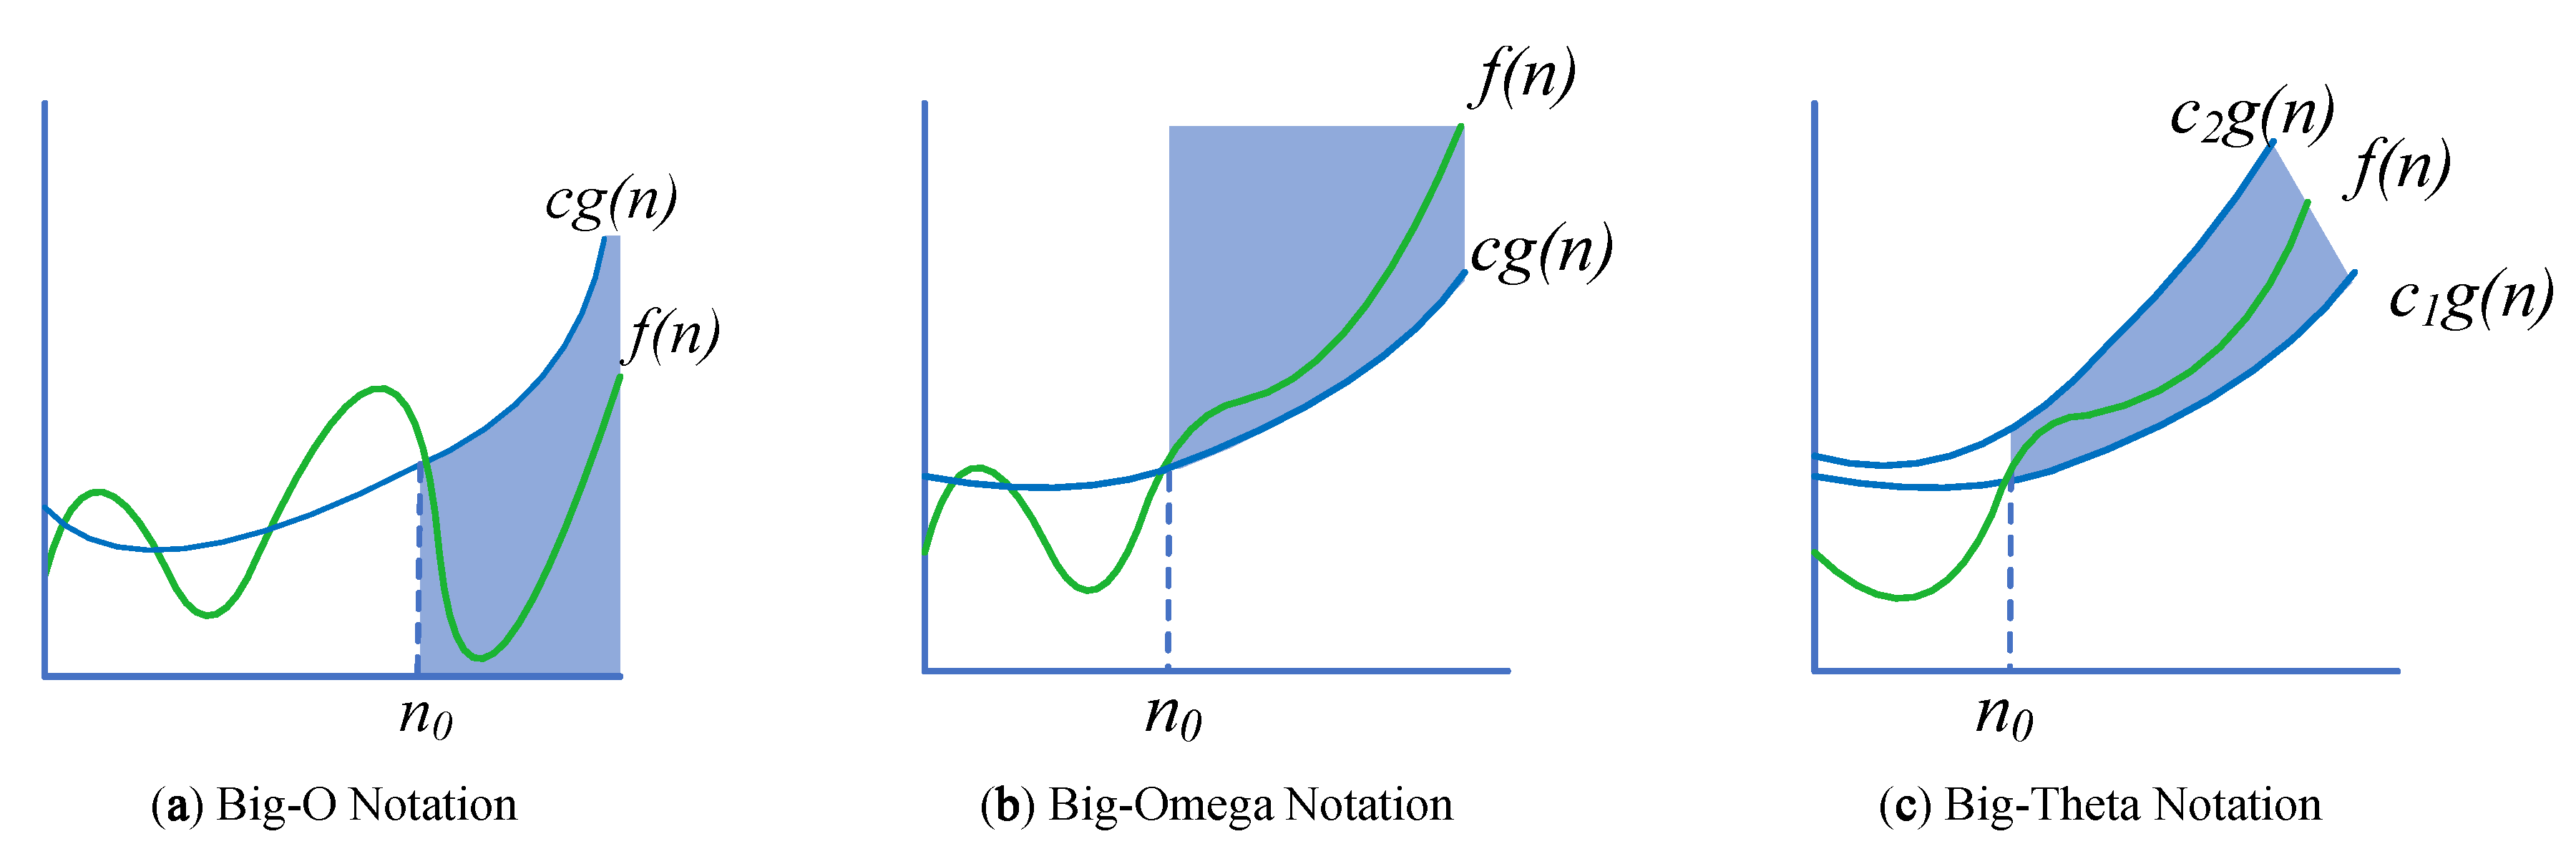
\includegraphics[width=\textwidth]{big.png}
		\caption{Asymptotic Notation
		\url{shorturl.at/xAFQ1}}
		\end{center}
		\end{figure}
\subsection{Little-oh}

\defn{$o(g(n))$}{$\lim_{n\to\infty}\frac{f(n)}{g(n)} = 0$}

\par{We say that $f(x)$ is $o(g(x))$ if $g(x)$ grows much faster than $f(x)$,
i.e. if $f(n)$ is $O(g(n))$ and $f(n)$ is not $\Omega(g(n))$}


\subsection{Computing Running Times}

	\par{The following, follows from the propositions above}

	\begin{enumerate}
			\item\textbf{Loops : } at most the running time of its contents times
					the number of iterations
			\item\textbf{Nested Loops : } it should be analysed inside out. Take
					the runtime of the expression and multiply it by the product
					of of the sizes of all the loops
			\item\textbf{Consecutive Statements : } add
			\item\textbf{If-then-else : } at most the time of the test condition
					with the maximum of the running times of the two branches
	\end{enumerate}

	\example{

		\begin{lstlisting}
			sum = 0;
			for (i=1; i<=n; i++)
				sum += n;
		\end{lstlisting}



	\par{See more examples
	\href{https://opendsa-server.cs.vt.edu/ODSA/Books/CS2/html/AnalProgram.html}{here}}
	}
\subsubsection{Analysis of Insertion-Sort}
	\example{Insertion-Sort \\
	\begin{algorithm}[H]
	\DontPrintSemicolon
	\SetAlgoLined\KwData{Array of integers : A}
	\SetKwFunction{KwFn}{Insert}
	\KwResult{Permutation of A such that A[0] $\leq$ A[1] $\leq \dots$ A[n-1] }
	\KwFn{A}\\
	\For{$j=1$ \KwTo $n-1$}{\tcc*[r]{$n$}
	    key := A[j]\tcc*[r]{$n-1$}\;
	    i := j-1\tcc*[r]{$n-1$}\;
	    \While{$i \geq 0$ {\bf and} $A[i] > key$}{\tcc*[r]{$\sum_{1}^{n-1}t_j$}
	        A[i+1] := A[i]\tcc*[r]{$\sum_{1}^{n-1}(t_{j}-1)$}\;
	        i := i-1\tcc*[r]{$\sum_{1}^{n-1}(t_{j}-1)$}\;
	    }
	    A[i+1] := key\tcc*[r]{$n-1$}\;
	}
		\caption{Insertion-Sort}
	\end{algorithm}
	\vspace{3mm}
	\par{Hence, summing the individual operations $$T(n) = n + (n-1) + (n-1)  + \sum_{1}^{n-1}t_{j} + \sum_{1}^{n-1}(t_{j}-1) + \sum_{1}^{n-1}(t_{j}-1) + (n-1)$$ }

	\par{\textbf{Best Case:} $A$ is already sorted , which means that the while loop is never executed and $t_j = 1$. Hence,
	$$ T(n) = n + (n-1) + (n-1)  + (n-1) + 0 + 0 + (n-1) = O(n)$$}

	\par{\textbf{Worst Case:} At every iteration we shift $j$ elements : $t_j = j$. So,
		$$\sum_{1}^{n-1}t_{j} = \sum_{1}^{n-1}j = \frac{n(n-1)}{2} = O(n^2)$$
		$$\sum_{1}^{n-1}t_{j}-1 = \sum_{1}^{n-1}(j-1) = \frac{n(n-1)}{2} - (n-1) = O(n^2)$$
		Hence,
		$$T(n) = n + (n-1) + (n-1)  + O(n^2) + O(n^2) + O(n^2) + (n-1) = O(^2)$$
	}
}
